\documentclass[a4paper, openright, 12pt]{article}
\usepackage[spanish]{babel}
\usepackage[utf8]{inputenc}
\usepackage{setspace}
\usepackage{url}
\usepackage{hyperref}
\usepackage{enumerate}
\usepackage{blindtext}
\usepackage{graphicx}
\graphicspath{ {../imgs/} }

\author{Grupo de trabajo PAPIME}
\date{ENERO 2017}

\begin{document}


\begin{titlepage}

    \begin{center}
        \vspace{-1in}
        \vspace{0.35in}

        \begin{large}
            UNIVERSIDAD NACIONAL AUTÓNOMA DE MÉXICO
            \vspace{0.75in}

            FACULTAD DE PSICOLOGÍA
            \vspace{0.95in}

            GUÍA DE INSTALACIÓN DE SOFTWARE DE APOYO A LA DOCENCIA PARA EL CURSO \textit{APRENDIZAJE Y CONDUCTA ADAPTATIVA I}

            \vspace{4.5in}
            \rule{110mm}{0.02mm}


            \vspace{0.25in}
            Enero 2017
        \end{large}


    \end{center}

\end{titlepage}


\tableofcontents
\newpage{}

\section{Introducción}
    Este documento tiene como objetivo ayudar a los alumnos del curso Aprendizaje y Conducta Adaptativa I (ACA I) con el proceso de instalación del software necesario para trabajar con el lenguaje de programación Python. Es importante mencionar que el material de apoyo para el curso \textit{ACA I} está desarrollado en el lenguaje de programación Python 2.7, esta guía tiene el proposito de descargar e instalar el conjuto de librerías necesarias para ejecutar dicho material de trabajo.\\

    Será necesario para el alumno contar con una computadora, conexión a internet y mucha paciencia. Hemos dividido el documento en tres secciones, cada una de ellas corresponde a cada uno de los sistemas operativos más usados: Windows, Ubuntu (linux) y MAC os. La estructura del documento ayudará al alumno a dirigirse únicamente a la sección que corresponde al sistema operativo instalado en su computadora y seguir una serie de pasos que confiamos lo llevarán a buen puerto.\\

    Es muy importante para los redactores de tal documento que este sea claro para el alumno. Por lo tanto se pide al lector que cualquier comentario o sugerencia se haga llegar a los datos de contacto que aparecen a continuación.

\newpage{}



%Sección de instalación en Windows....
  \section{Preparando la instalación}
    Por lo que sabemos Windows es, quizá, el sistema operativo más conocido y usado en la actualidad. Los procedimientos que se describen a continuación fueron probados en los sistemas operativos Windows 7 y Windos 10, por lo cual sugerimos al lector identicar la version de sus sistema operativo así como el tipo de sistema que tiene.\\

    Comenzaremos por revisar estas dos características del sistema operativo instalado en la cumputadora del lector, puesto que en un futuro será indispensable conocer esta información.\\

    \begin{itemize}

      \item{El primer paso será ir al menu de Inicio de windos, seleccionar la opción \textit{Equipo}.}

      \begin{figure}[ht]
        \centering
        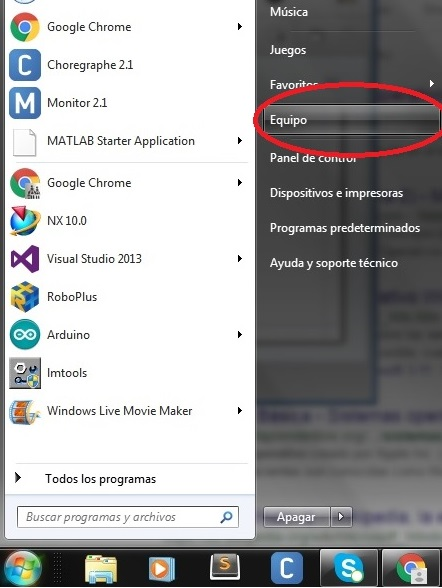
\includegraphics[width=3.5cm, height=5cm]{/w_1.jpg}
      \end{figure}

      \item{Posteriormente, en la parte superior de la venta seleccionar la opción \textit{Propiedades del sistema}.}\\

      \begin{figure}[ht]
        \centering
        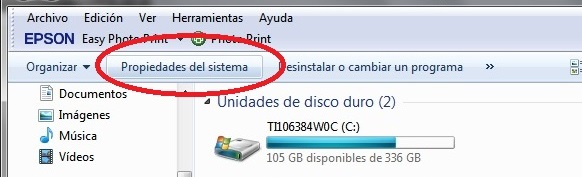
\includegraphics[scale=0.4]{/w_2.jpg}
      \end{figure}

    \end{itemize}

    En la nueva ventana podemos ver las características del equipo: la versión de Windows, el tipo de sistema, el tamaño de la memoria RAM, el tipo de procesador entre otras. Las características que son de nuestro interés son la versión del sistema operativo y el tipo de sistema.\\

    \begin{figure}[ht]
    \centering
    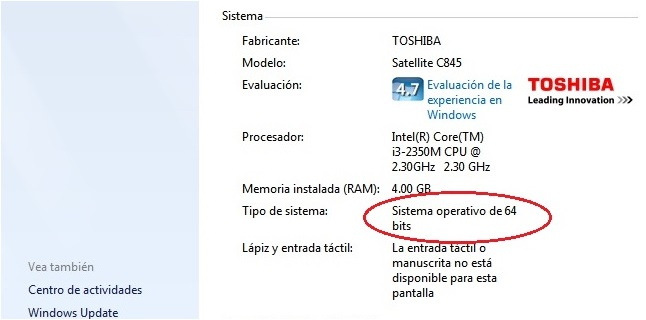
\includegraphics[scale=0.5]{/w_3.jpg}
    \end{figure}

    Recomendamos al lector tener en cuenta esta información o de ser necesario tomar nota, la información deberá observarse de esta manera:\\

    \textit{  Tipo de sistema: Sistema operativo de \textbf{64bits}}\\

    En este punto tenemos la información de nuestro sistema operativo, esta información es importante ya que de ello dependerá las librerías que descarguemos.

    \newpage{}





  \section{Windows  y MAC os}
    La manera más fácil de instalar los paquetes necesarios para ejecutar los códigos de python es instalar el IDE de desarrollo llamado \textit{Spyder}.\\

    Una de las formas más eficientes de instalar Spyder es a través de \textit{Anaconda}. Recapitulando y a fin de no confundir más al alumno: Anaconda es una plataforma abierta enfocada a la ciencia de datos. \textit{Anaconda} incluye a su vez \textit{Spyder} que es una interfaz gráfica basada en Python la cual nos permite visualizar la consola, el editor de código, el visualizador de variables, entre otras.\\

    Por tanto el primer paso será instalar Anaconda.\\

      \begin{enumerate}
        \item{Para instalar Anaconda debemos ir al siguente link: \url{https://www.continuum.io/downloads} }
        \item{Una vez allí seleccionamos la opción correspondiente a nuestro sistema operativo \textbf{(Windows, Linux o MAC os)} y a la versión de \textbf{Python 2.7}.}\\

        \begin{figure}[ht]
          \centering
          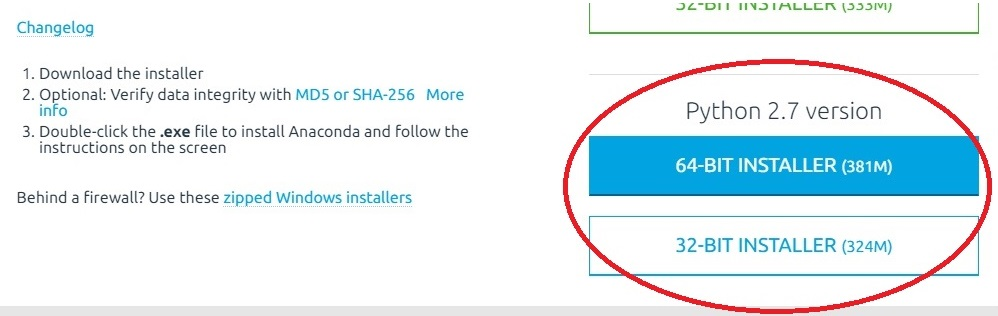
\includegraphics[scale=0.5]{/w_4.jpg}
        \end{figure}

        \item{Dependerá de las características de nuestra computadora si seleccionamos la opción de 32-bits o de 64-bits.}

        \item{Una vez concluida la descarga procedemos a instalar el ejecutable.}\\

        \item{Por lo que corresponde al los sistemas operativos Windows y MAC instalar software no tiene mayor complejidad que ejecutar el instalador gráfico.}

        \item{Pondremos especial atención a la ventana: \textit{Advanced installation Options}. En la cual nos aseguraremos de habilitar las \textbf{dos opciones} que nos muestra el instalador.}

        \begin{figure}[ht]
          \centering
          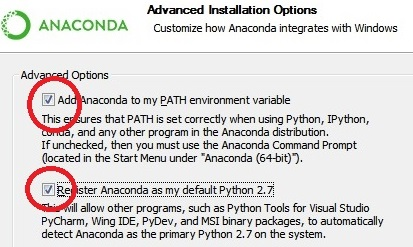
\includegraphics[scale=0.8]{/w_15.jpg}
        \end{figure}

        \item{Y listo solo esperemos a que el software termine de instalarse.}
        \begin{figure}[ht]
          \centering
          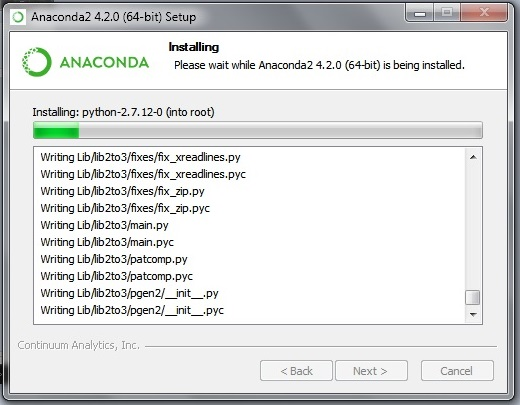
\includegraphics[scale=0.4]{/w_10.jpg}
        \end{figure}

      \end{enumerate}

      Una vez instalado Anaconda podemos buscarlo en nuestros programas en el menú principal de Windows. Y deberíamos observar una interfaz parecida a la mostrada en la figura.\\
      \begin{figure}[ht]
        \centering
        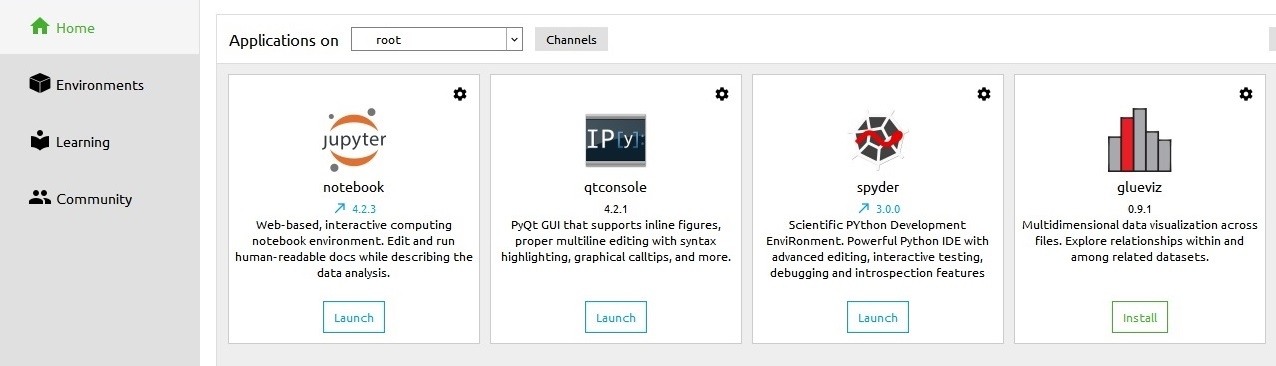
\includegraphics[scale=0.45]{/w_11.jpg}
      \end{figure}
      \vspace{0.35in}

\newpage{}
\newpage{}



%Sección de instalación en Linux....
  \section{Linux}
    En lixun basta con abrir una terminal y teclear los comandos:\\
    \begin{itemize}
      \item{\textit{sudo apt-get update}}\\
        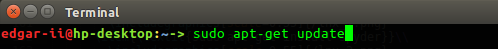
\includegraphics[scale=0.75]{/lnx_1.png}
      \item{\textit{sudo apt-get install spyder}}\\
        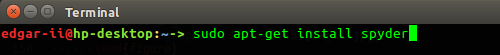
\includegraphics[scale=0.75]{/lnx_2.png}
    \end{itemize}
  \newpage{}





  \section*{Apéndice}
    \subsection*{Configuración del entorno de trabajo}

      Procedemos a ejecutar \textit{Spyder}. El siguiente paso será configurar el entorno de trabajo de Spyder para tener una experiencia óptima al ejecutar y desarrollar los códigos proporcionados en el material de apoyo.\\

      Para ello iremos a la opción de \textit{Herramientas} y posteriormente el menú de preferencias. Como se muestra a continuación.\\
      \begin{figure}[ht]
        \centering
        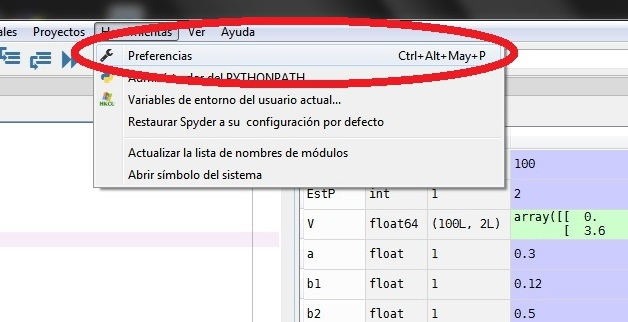
\includegraphics[scale=0.55]{/config_2.jpg}
      \end{figure}

      Allí configuraremos la opción \textit{Ejecutar} como se muestra a continuación.
      \begin{figure}[ht]
        \centering
        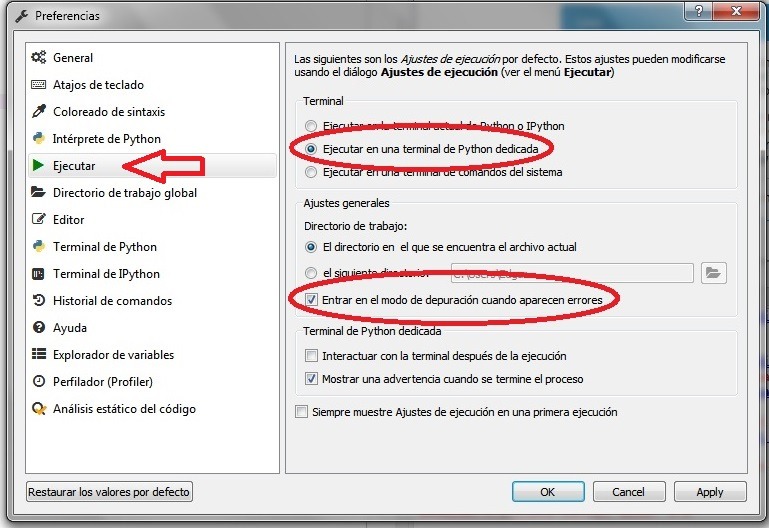
\includegraphics[scale=0.5]{/config_3.jpg}
      \end{figure}

      Continuando con el proceso verificaremos que la configuración se haya realizado de maner adecuada, por tanto daremos click en la opción preferencias de ejecución y verificaremos que las configuraciones son las mismas.

      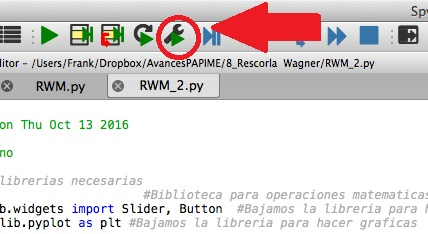
\includegraphics[scale=0.5]{/config_1.jpg}
      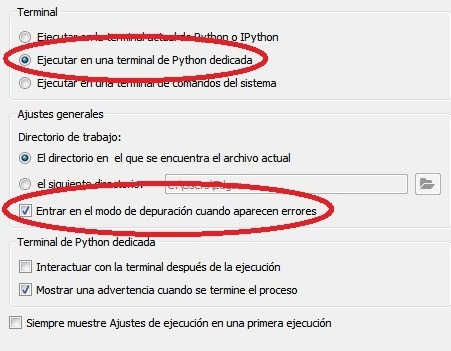
\includegraphics[scale=0.5]{/config_4.jpg}\\

      Lo que resta hacer es abrir alguno de los códigos proporcionados en el material de apoyo y ejecutarlo dando click en la flecha verde de la parte superior. Deberá desplegarse una ventana con una bonita gráfica.\\

      Listo tenemos todo lo necesario para comenzar a trabajar con códigos escritos en \textit{Python}. Reiteramos la necesidad de obtener retroalimentación de los alumnos y usuarios con el fin de mejorar el material de apoyo, por tanto si usted presentó alguna dificultad al seguir esta guía o los resultados no son los esperados le pedimos ponerse en contacto con los colaboradores de este proyecto para brindarle el soporte técnico necesario.
  \newpage{}


  \section*{Datos de contacto}
    \begin{itemize}
      \doublespacing
      \item{\textit{Adriana Felisa Chávez De la Peña} - \url{ adrifelcha@gmail.com} }
      \item{\textit{Edgar de Jesús Vázquez Silva} - \url{edgarvazquez1403@gmail.com} }
      \item{\textit{Marco Antonio Negrete Villanueva} - \url{mnegretev@gmail.com} }
    \end{itemize}

\end{document}
